\documentclass[10pt,hyperref={pdfpagemode=FullScreen},aspectratio=169]{beamer}

\usetheme[progressbar=frametitle]{metropolis}
\usepackage{appendixnumberbeamer}
\usepackage{lipsum}
\usepackage{amsmath}
\usepackage{amssymb}
\usepackage{booktabs}
\usepackage{siunitx}
\usepackage[scale=2]{ccicons}
\usepackage{pgfplots}
\usepgfplotslibrary{dateplot}
\usepackage{tikz}
\usetikzlibrary{positioning, shapes.geometric}
\pgfplotsset{compat=newest} % Allows to place the legend below plot
\usepgfplotslibrary{units} % Allows to enter the units nicely
\usepackage{circuitikz}
\usetikzlibrary{shapes,arrows}
\usepackage{dirtytalk}
\usepackage{xspace}




% Bibliography
\usepackage[
    backend=biber,
    style=ieee,
    natbib=true,
    url=false, 
    doi=true,
    eprint=false
]{biblatex}
%\addbibresource{references.bib}


\newcommand{\themename}{\textbf{\textsc{metropolis}}\xspace}
\newcommand{\universidade}{University of Brasília}
\newcommand{\doctitle}{Signal and Power Integrity}

\definecolor{mpigreen}{HTML}{007977}
\setbeamercolor{frametitle}{bg=mpigreen}

\title{\doctitle}

\author{Daniel Araújo}
\institute{\universidade}
\titlegraphic{\hfill
\includegraphics[height=1.5cm]{../logo}}

\title{Introduction to Signal Integrity}

\author{Prof. Daniel Costa Araújo}

\usepackage{graphicx}
\usepackage{subfigure}
\usepackage{verbatim}
\begin{document}


\frame{\titlepage}

  
  \begin{frame}
    \frametitle{Outline}
    \tableofcontents
  \end{frame}
  
\section{Introduction}


\frame{
   \frametitle{Signal Integirty, Power Integrity, Eletromagnetic Compatibility}

\begin{block}{Why study?}
  In the past, when 10-MHz clock frequencies were common, interconnects were not a major concern for system performance. However, as clock frequencies increased and signal rise times decreased, signal integrity (SI), power integrity (PI), and electromagnetic compatibility (EMC) became important factors in the design of electronic products.
\end{block}

\begin{block}{Definition}

  \begin{itemize}
    \item Signal integrity (SI) deals with signal distortion;
    \item power integrity (PI) addresses noise on interconnects and power delivery components; \item electromagnetic compatibility (EMC) involves the product's radiated emissions and susceptibility to external electromagnetic interference.
  \end{itemize}
  
\end{block}

}


\begin{frame}
  \frametitle{Main problems in the Field}

  \begin{itemize}
    \item Signal distortion on one net
    \item Rise-time degradation from frequency-dependent losses in interconnects
    \item Cross talk between two or more nets
    \item Ground and power bounce as a special case of cross talk
    \item Rail collapse in power and ground distribution
    \item Electromagnetic interference and radiation from the entire system
\end{itemize}

\begin{block}{NOTE}
  Understanding the root cause of these six families of problems and the essential principles behind them helps to find and fix issues in each family, ensuring successful product design.
\end{block}
\end{frame}


\section{Signal distortion in net}

\begin{frame}
  \frametitle{Understanding a Single Net}
      \begin{itemize}
          \item A single net is a group of interconnected metal traces or conductors in an electronic system.
          \item Electrically connects components (e.g., output pins, input pins) on a printed circuit board (PCB) or within an electronic system.
          \item Comprises both the signal path and the return path for the signal current.
      \end{itemize}
      \begin{figure}
          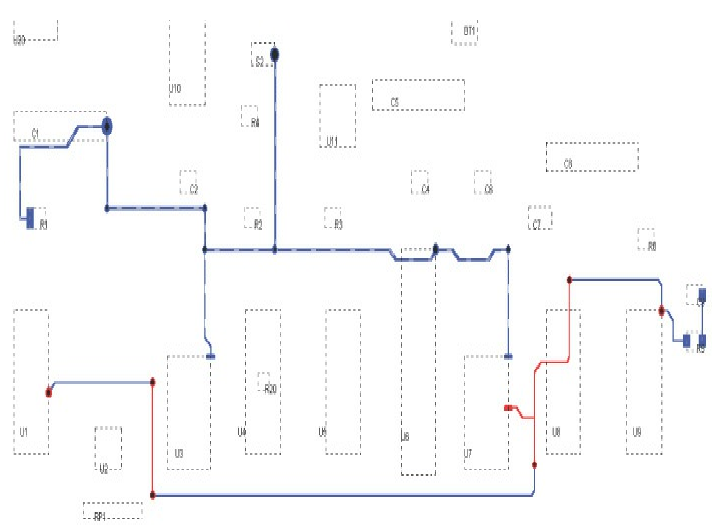
\includegraphics[scale=0.3]{Fig/two_nets.png}
          \caption{}
      \end{figure}
  \end{frame}


  \begin{frame}{Understanding Signal Propagation and Impedance Discontinuities}
    \begin{enumerate}
      \item Signal leaves output driver as voltage and current.
      \item Signal encounters interconnect, perceived as electrical impedance.
      \item Signal continuously assesses instantaneous impedance.
      \item Constant impedance ensures undistorted signal propagation.
      \item Impedance changes cause signal reflection and distortion.
      \item Distortions may lead to false triggering.
      \item Discontinuities: features that change the net's cross-section or geometric shape.
      \item Discontinuities distort the signal from its original form.
    \end{enumerate}
  \end{frame}



\begin{frame}{Impedance Discontinuities and Signal Integrity}
  \begin{itemize}
    \item Features changing impedance include:
      \begin{itemize}
        \item End of interconnect
        \item Line-width change
        \item Layer change through a via
        \item Gap in return-path plane
        \item Connector
        \item Routing topology change (branch, tee, stub)
      \end{itemize}
    \item Discontinuities arise from cross-section changes, routing topology, or added components.
    \item Common discontinuity: end of a trace (high or low impedance).
    \item Solution: Engineer the interconnect impedance to be constant.
  \end{itemize}
\end{frame}


\begin{frame}
  \frametitle{Best Practices}

  \begin{enumerate}
    \item Use a board with constant, or “controlled,”
    impedance traces. This usually means using uniform
    transmission lines.
    \item To manage the reflections from the ends, use a
    termination strategy that controls the reflections by
    using a resistor to fool the signal into not seeing an
    impedance change.
    \item Use routing rules that allow the topology to
    maintain a constant impedance down the trace. This
    generally means using point-to-point routing or
    minimum-length branch or short stub lengths.
    \item Engineer the structures that are not uniform
    transmission lines to reduce their discontinuity.
    This means adjusting fine geometrical design
    features to sculpt the fringe fields.
  \end{enumerate}


\end{frame}


\section{Cross-talk}

\begin{frame}{Cross Talk in Different Environments}
  Cross talk occurs in two different environments:
  \begin{itemize}
    \item When the interconnects are uniform transmission lines, as in most traces in a circuit board.
    \item When they are not uniform transmission lines, as in connectors and packages.
  \end{itemize}
  In controlled-impedance transmission lines where the traces have a wide uniform return path, the relative amount of capacitive coupling and inductive coupling is comparable. In this case, these two effects combine in different ways at the near end of the quiet line and at the far end of the quiet line.

  \begin{figure}
    \centering
    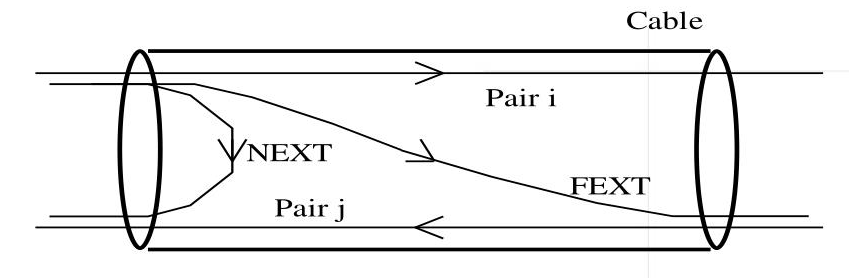
\includegraphics[width=0.5\textwidth]{Fig/near_far.png}
    \caption{Measured near- and far-end cross talk between two nets in a circuit board.}
  \end{figure}

\end{frame}
  

\begin{frame}{Cross Talk and Coupled Noise}
  \begin{itemize}
    \item Lowest cross talk configuration: wide uniform plane as return path.
    \item Deviation from this configuration increases coupled noise.
    \item Inductively coupled noise dominates, causing switching noise, delta I noise, dI-dt noise, ground bounce, SSN, and SSO noise.
    \item Generated by mutual inductance.
    \item Occurs mainly in connectors, packages, and vias where return path conductor isn't a wide, uniform plane.
    \item Ground bounce: special case of cross talk with overlapping return currents in the same conductor, leading to high mutual inductance.
  \end{itemize}
\end{frame}

\section{Rail collapse noise (Power supply-induced noise)}


\begin{frame}
  \frametitle{Definition}

  \begin{block}{When happens?}
    \begin{itemize}
      \item occurs when the voltage rails in an integrated circuit (IC) experience voltage fluctuations due to the simultaneous switching of many digital components within the circuit.
      \item voltage fluctuations can cause errors, affect performance, or even lead to complete system failure.
    \end{itemize}
  \end{block}
\end{frame}

\begin{frame}
  \frametitle{How to mitigate}

\begin{enumerate}
  \item Decoupling Capacitors:
  Place decoupling capacitors close to the power supply pins of the IC. These capacitors act as local energy reservoirs that can quickly supply the additional current required during transient events, helping to stabilize the voltage rail. Decoupling capacitors should be chosen based on their capacitance value, equivalent series resistance (ESR), and equivalent series inductance (ESL) to ensure optimal performance in the target frequency range.
  \item Voltage regulator selection:
  Choose voltage regulators with low output impedance and fast transient response, which can better handle sudden changes in load current and minimize voltage fluctuations. Switching regulators like voltage regulator modules (VRMs) are generally more efficient and have better transient response compared to linear regulators like low-dropout regulators (LDOs).
  \item Grounding:
  Use a solid ground plane to provide a low-impedance return path for currents, which helps reduce noise coupling. Connect all ground points to the ground plane using short, direct paths. For mixed-signal designs, use a partitioned ground plane to separate analog and digital grounds, connecting them at a single point to avoid ground loops
\end{enumerate}


\end{frame}

\end{document}
